\chapter{Software Design}

This section will discuss the Software and Firmware implementation of Verified
Boot. 
Verified Boot (Vboot) is a secure boot implementation only runs code that has
been signed by Google and is untampered.
Images that have been recognized as security risks will not be loaded and the system will restart into a Recovery Mode.
Google has implemented different modes that Vboot can boot with and these modes alter the program flow and security guarantees.
In this section I will discuss the security promises made by the system as well
as the attack vectors that are not considered.
I will also discuss relevant data structures and program flow.

\section{Security Promises}

The main purpose of Chrome OS's verified boot is to provide relative security to the end user without sacrificing usability or functionality. 
In its mission statement, verified boot is designed against an ``opportunistic hacker''~\cite{vboot-design-doc}.
Vboot protects against vectors of attack that are relatively quick to exploit.
Vboot will realize any attack or modification on the next boot cycle.
Once an attack is realized Vboot will get the system back to a secure state.
An example of an attack that would be caught by Vboot would be the installation
of a malicious kernel driver to act as a keylogger, or the replacement of the
current kernel with an older version that has known vulnerabilities.

There are many attacks that Vboot is not able to recognize or protect against.
For example, Vboot does not make any promises to the safety of the system once the kernel is running and the user has control. 
Any attacks that are outside of the kernel (in userspace) would remain
undetected because they would not modify the kernel.
For example, changing the Web browser to use a proxy that collects information
would not be considered a kernel attack.
Userspace programs by definition have less access to the system and this reduces the severity and influence of the attack.
Possibly one of the biggest flaws is that any attack to the kernel during
runtime would remain until the system was powered down.
In certain situations could provide plenty of time for an attack to steal valuable data.
However, such an attack is outside the scope of this paper.

\section{Verified Boot Flow}

In order to divide the code modularly and have Verified Boot be extensible for current and future platforms, Google has split the process into three main sections as seen in Figure~\ref{fig:vboot_stages_overview}.
This also allows Google to make the Read-Only stage as small as possible, which is good because bugs in this stage cannot be fixed.
These sections are referred to as Read-Only (RO) Firmware, Read-Write
(RW) Firmware, and Kernel.
These sections are run in sequence with each section verifying the section that comes later.
In this way the root of trust starts from the Read-Only portion and builds until the system has booted completely.
For the scope of this document we will discuss only the Verified Boot process for the verification between RO Firmware and RW Firmware. 
This verification contains more interesting control flow, and process is essentially repeated for the verification between the RW Firmware and the Kernel.

\begin{figure}
\begin{subfigure}{.4\textwidth}
  \centering
  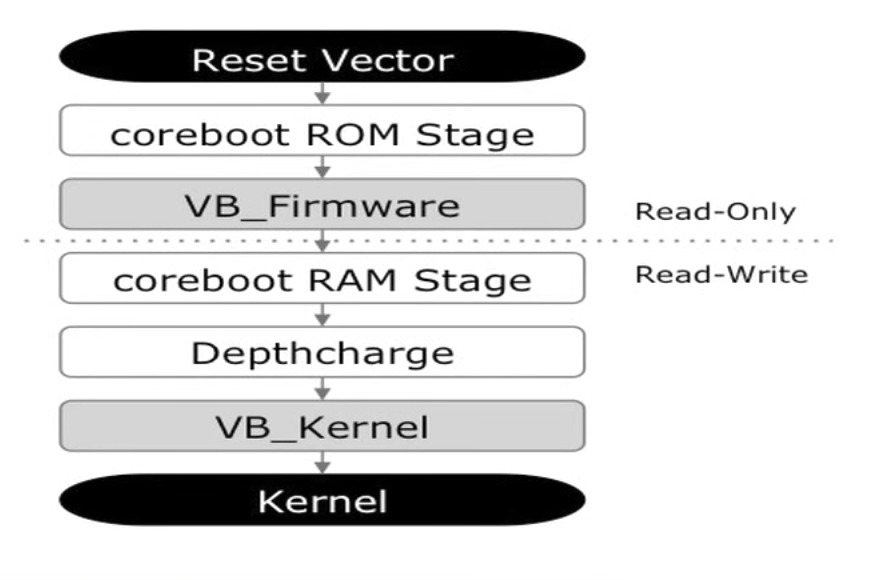
\includegraphics[width=1.0\linewidth]{vboot_stages_overview.png}
\end{subfigure}
\begin{subfigure}{.60\textwidth}
  \centering
  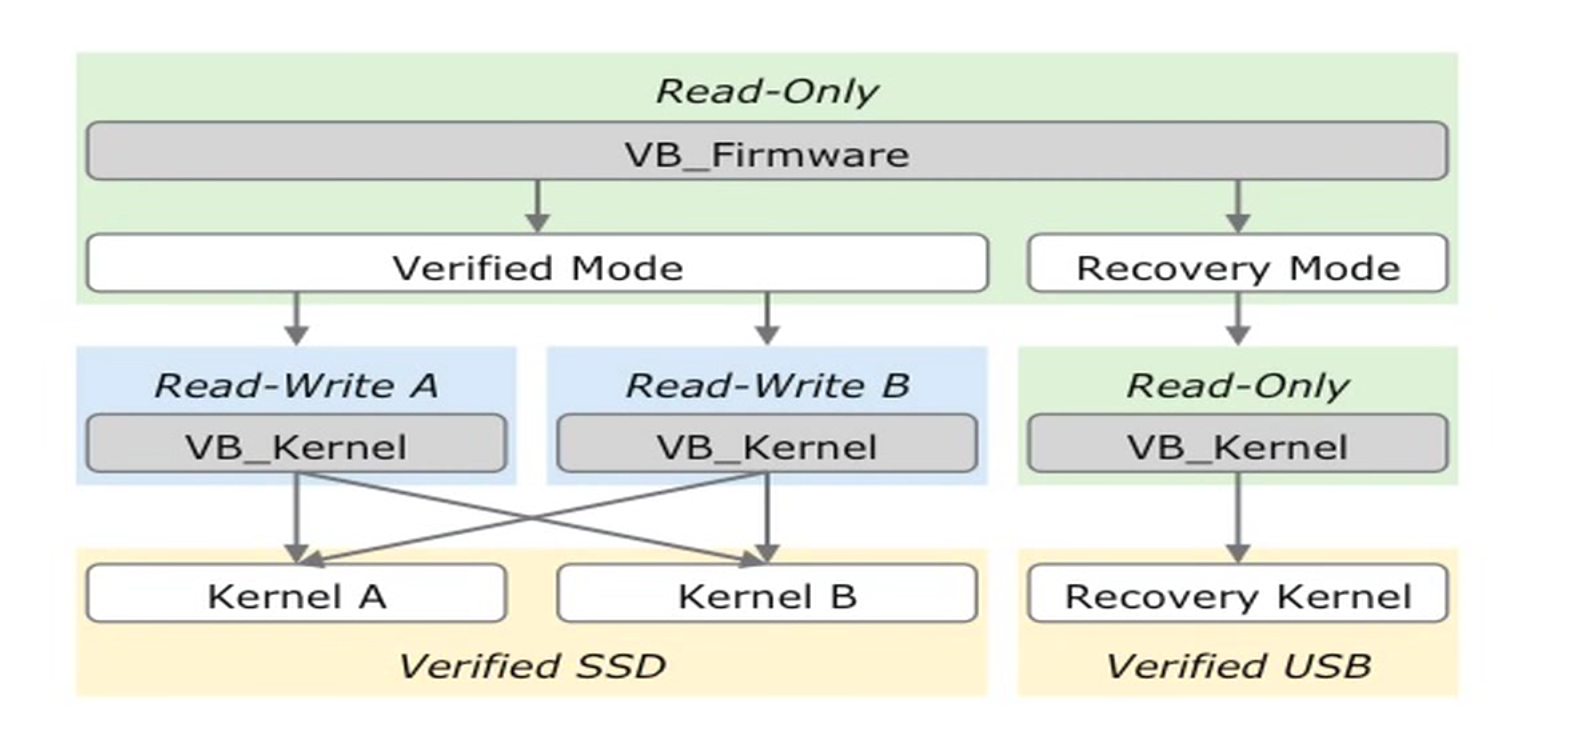
\includegraphics[width=1.0\linewidth]{vboot_stages_AB_recovery.png}
\end{subfigure}
\caption{The left image shows the stages of Vboot Firmware. The right image
shows the different boot paths, and data locations. Both make the distinction
between Read-Only and Read-Write memory.}
\label{fig:vboot_stages_overview}
\end{figure}

The RO Firmware runs first and as such is the root of trust for the entire platform.
It is responsible for verifying the RW Firmware image and it contains all of the code and hardware drivers it needs to accomplish this task.
It verifies the RW Firmware Image signature using Google's main public key.
This public key is packaged with the RO Firmware and is also read only so it is guaranteed to be secure.
The RO Firmware is also responsible for handing the main control of Vboot, and this includes the transitions between Developer Mode, Safe Mode, and Recovery Mode.
These transitions will be described in more detail in Section~\ref{sec:boot-modes}.

\begin{figure}
  \centering
  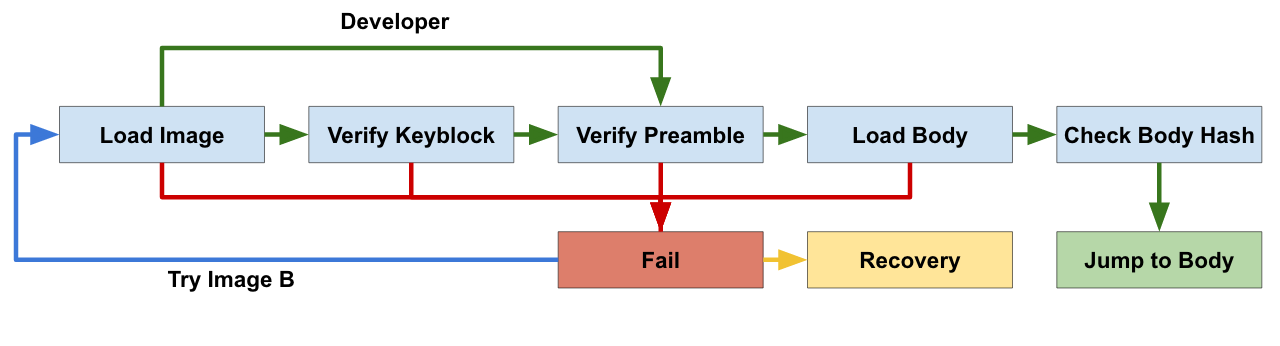
\includegraphics[width=0.8\linewidth]{verification_flow.png}
  \caption{The logical flow for verifying the firmware image. Notice
  the different path for Developer mode, and the possibilities for
  failure.}\label{fig:verif_flow}
\end{figure}

The stages that the RO Firmware goes through include loading the image, verifying the keyblock, verifying the preamble, loading the body, verifying the body, and then executing the code in the body. 
These stages can be seen in Figure~\ref{fig:verif_flow}.

Loading the image consists of copying the image out of the Flash Memory (Section~\ref{flash_mem}) and into RAM where pointers to the image are passed around on the C call stack.
Verifying the Keyblock consists of using its signature, which is a hash of its full information that is signed by Google's Private key.
Google's Public Key, which is stored in Read-Only Memory, is used to decrypted the signature, so that it is now only a hash of the Keyblock.
Finally, the entire Keyblock is hashed, and the two are compared.
If the hashes are not equal, then the Keyblock currently viewed by the machine is not the one that was originally signed by Google.

The Preamble is verified in the same way, except that a different Private and Public Key pair is used.
The Keyblock holds the key that is used for the Preamble's signature.
The Keyblock is used so that Google has the ability to change the encryption
type of the Preamble and Firmware if they wish.
Google's Main Public Key is stored in Read-Only memory, so it cannot be changed.
This hierarchy of keys also allows Google to be less careful with their ``lower
security'' keys because they can change them via update if the key is
compromised.

After the Preamble is verified, the Firmware Image is hashed and compared
against the hash stored in the preamble. 
The hash in the preamble has already been verified because the preamble was
signed, so this verifies that the Image is correct and unmodified. Finally, the
system jumps to the Image and begins to execute the code for the main Firmware
and Operating System.


\section{Boot Modes}\label{sec:boot-modes}

Vboot has three major boot states that influence the program's behavior.
The first state is the Secure state which goes through the full process of Verified Boot normally.
The second state is the Recovery state which allows for a broken machine to
format all memory and revert to a secure state.
The third state is the Developer state and in this state the RSA signature is not verified.
The Developer state exists so that hobbyists can write their own firmware boot code and run operating systems other than Chrome OS\@.

The transitions allowed between the states can be seen in
Figure~\ref{fig:mode_fsm}.
On each transition, Vboot is responsible for taking steps to ensure that
security is preserved. 
These responsibilities are also seen in the figure.

\begin{figure}
  \centering
  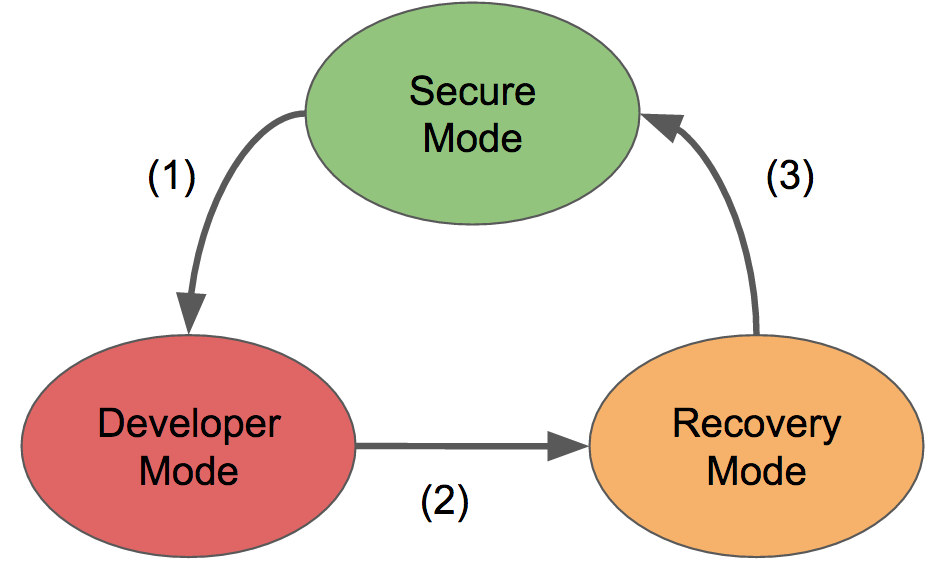
\includegraphics[width=0.4\linewidth]{mode_fsm.png}
  \caption{The FSM for the boot modes. \\
  1. The TPM's nonvolatile storage and keys are wiped. The user's data
  is erased. \\
  2. The laptop is booted into Recovery, Vboot installs a Chrome USB.
  \\
  3. The TPM's storage goes through reconfiguration. The entire disk is wiped.
  \\}\label{fig:mode_fsm}
\end{figure}

\subsection{Developer Mode}

Developer mode poses interesting security questions to Verified boot because it essentially disables the security guarantees and allows the system to move into an insecure state~\cite{developer-mode}. 
There are various security requirements around the Developer state transition.
First, a physical presence is required to fully complete the developer mode transition. 
This means that a person must sit at the computer once it has been rebooted and press a certain key combination (Control + D) when the developer mode screen appears.
The physical presence exists such that developer mode cannot be enabled through an off-site software attack without the user's knowledge.
The developer mode screen is referred to internally as the ``Scary Screen'', and its purpose is also to prevent users from being tricked into enabling developer mode by an external phishing party.
Once Developer Mode is enabled, the system can no longer claim guarantees about the boot process or its own secure storage.
In order to prevent an attacker from enabling Developer Mode so that they could read secure storage, Vboot wipes all secure storage on the transition into Developer Mode.
The secure storage that is wiped includes the RSA keys and various secrets stored in the TPM and the partion on disk where user data is stored.
Wiping this data on the transition is necessary to the confidentiality of the system and failure to do so is a security risk.

These precautions are also taken on the transition from Developer Mode to Safe Mode. 
If secure storage is left untouched moving from Developer Mode to Safe Mode, then an attacker would be able to place potentially malicious information in secure storage.
The assumptions that Google places on secure storage require that it can only be written to and read from by Google.
The platform will not be able to recognize if secure storage is in an insecure or malicious state and so wiping it is the easiest way to ensure that the platform has full control.
On the transition from Developer to Safe Mode, the system has to go through Recovery Mode.

\subsection{Recovery Mode}

Recovery Mode is responsible for getting the system back to a secure state.
Recovery Mode will be activated automatically when an error is recognized in Vboot.
This error could range from hardware failures to a corrupted image to a detected attack on the system.
When the system boots into Recovery it is for a Recovery Image stored on external memory, either on an SD card or a USB drive.
The path for recovery uses a different RSA key for modularity and this recovery key is also stored in Read Only Flash in order to be unmodifiable.
Once the recovery image is verified to be secure and unmodified, the image is loaded off of the external storage and it is used to replace the images currently stored on the device.
Recovery mode is also responsible for wiping secure memory, including the user's disk partition and TPM's secure storage.
If Recovery completes successfully, the system is in a secure state and Vboot can then continue safely.
From a user perspective, Recovery is an easy way to wipe the device and restore it to Factory Settings.
Recovery is also the only way to roll the device back to an early image, and this rollback is sometimes necessary if there are known problems with a newly uploaded image.

\section{Data Structures}\label{sec:data-structures}

To start understanding the Vboot verification process, it is necessary to talk about the data structures that are used throughout. 
These data structures are populated by the Firmware Image that is being
verified. 
Through this section I will start at the highest hierarchical level of data structure then explain the structures that are contained within.

\subsection{Firmware/Kernel Image}

\begin{figure}
    \centering
    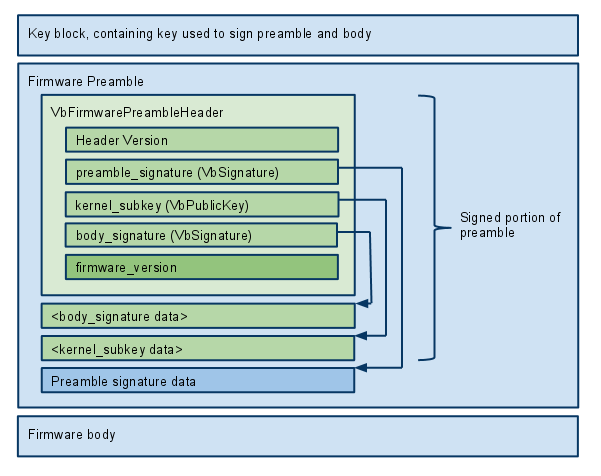
\includegraphics[width=0.6\linewidth]{fw_image.png}
    \caption{Layout of the Firmware Images~\cite{vboot-data-structures}}
    \label{fig:vboot_images}
\end{figure}

The actual image is not a data structure but a chunk of data that is stored contiguously in non-volatile memory.
The image structure, as seen in Figure~\ref{fig:vboot_images}, consists of three parts: a key block, a preamble, and the main body of the image.
The key block is verified first, and it is verified by the main RSA key stored in Read Only memory.
Once the key block has been shown to be safe, the RSA key located within will be used to verify the preamble.
The preamble contains the hash of the image's body.
The image's body contains the code that is going to be run next and it is checked against the hash stored in the preamble.
The preamble also contains the RSA key used to verify the key block of the Kernel image.

\subsection{Key Blocks}\label{sec:key_block}

\begin{figure}
\begin{subfigure}{.5\textwidth}
  \centering
  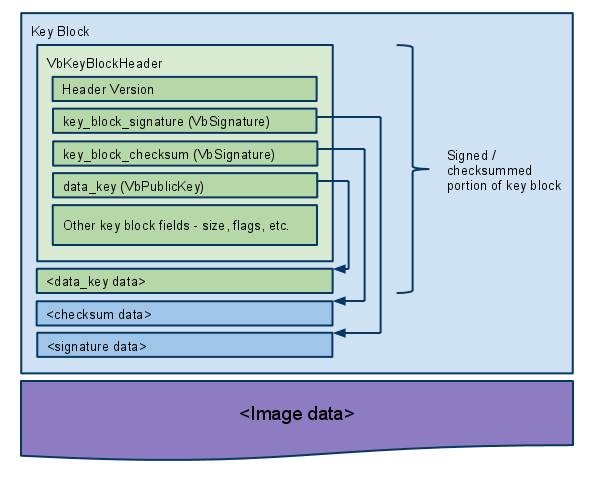
\includegraphics[width=1.0\linewidth]{vboot_keyblock.png}
\end{subfigure}
\begin{subfigure}{.20\textwidth}
  \centering
  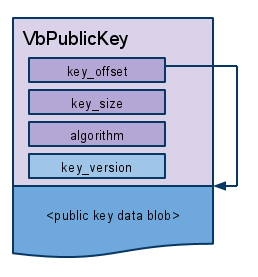
\includegraphics[width=1.0\linewidth]{vbpublickey.png}
\end{subfigure}
\begin{subfigure}{.20\textwidth}
  \centering
  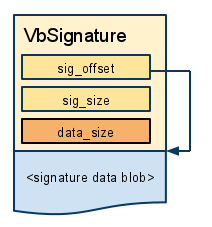
\includegraphics[width=1.0\linewidth]{vbsignature.png}
\end{subfigure}
\caption{The Keyblock data structure and Metadata for Keys and Signatures}
\label{fig:vboot_keyblock}
\end{figure}

The Key block is the first part of the image that is validated and it is used to validate the rest of the image.
The Key block is the data structure that allows a hierarchy of RSA keys to be used during Vboot.
Figure~\ref{fig:vboot_keyblock} shows the structure of the keyblock. 
The key block flags that are mentioned are used to determine which mode of Vboot the Keyblock is valid in. 
There are 4 possible boot modes corresponding to the combination of the two binary options, Developer and Recovery.
% info located in vboot_struct.h

Within the keyblock there exists data structures for a public key and a signature.
Google has added the ability to change their encryption strength.
They have added support for RSA 1024, 2048, 4096, 8192 and for SHA 1, 256, 512, for a total of 12 different possible algorithm combinations.

\subsection{Google Binary Block}

% info found in gbb_header.h
The Google Binary Block (GBB) is a part of Vboot's Root of Trust.
It is a data structure stored in Read-Only memory that is initialized and configured in the factory at the laptop's creation.
It contains the Root and Recovery RSA keys, a host of flags that affect boot operation, and the bitmaps used for various boot screens.


\section{Code Organization}

Like most modern operating systems, Chrome OS is written in C.
Like Linux, Chrome OS is maintained using Git for version control. 
Git is a diff-based, non-centralized version control system that makes it easy for programmers to share code, rollback changes, and maintain separate branches of the same codebase~\cite{git}.
Google has built a tool called ``repo'' that is used on top of git~\cite{repo}. 
Repo is a tool to manipulate multiple code repositories. 
It's primary benefit is that it allows a company to specify how multiple git repositories should be installed and placed within a given file-system.
This is both helpful and necessary as Chrome OS consists of over one thousand different external and internal repositories. 

Coreboot, vboot\_reference, depthcharge, are the repositories used for the firmware boot process.
The flow of Verfied Boot through the repos can be seen in
Figure~\ref{fig:code_repos} and the purpose of each repo is described below.

\begin{figure}
  \centering
  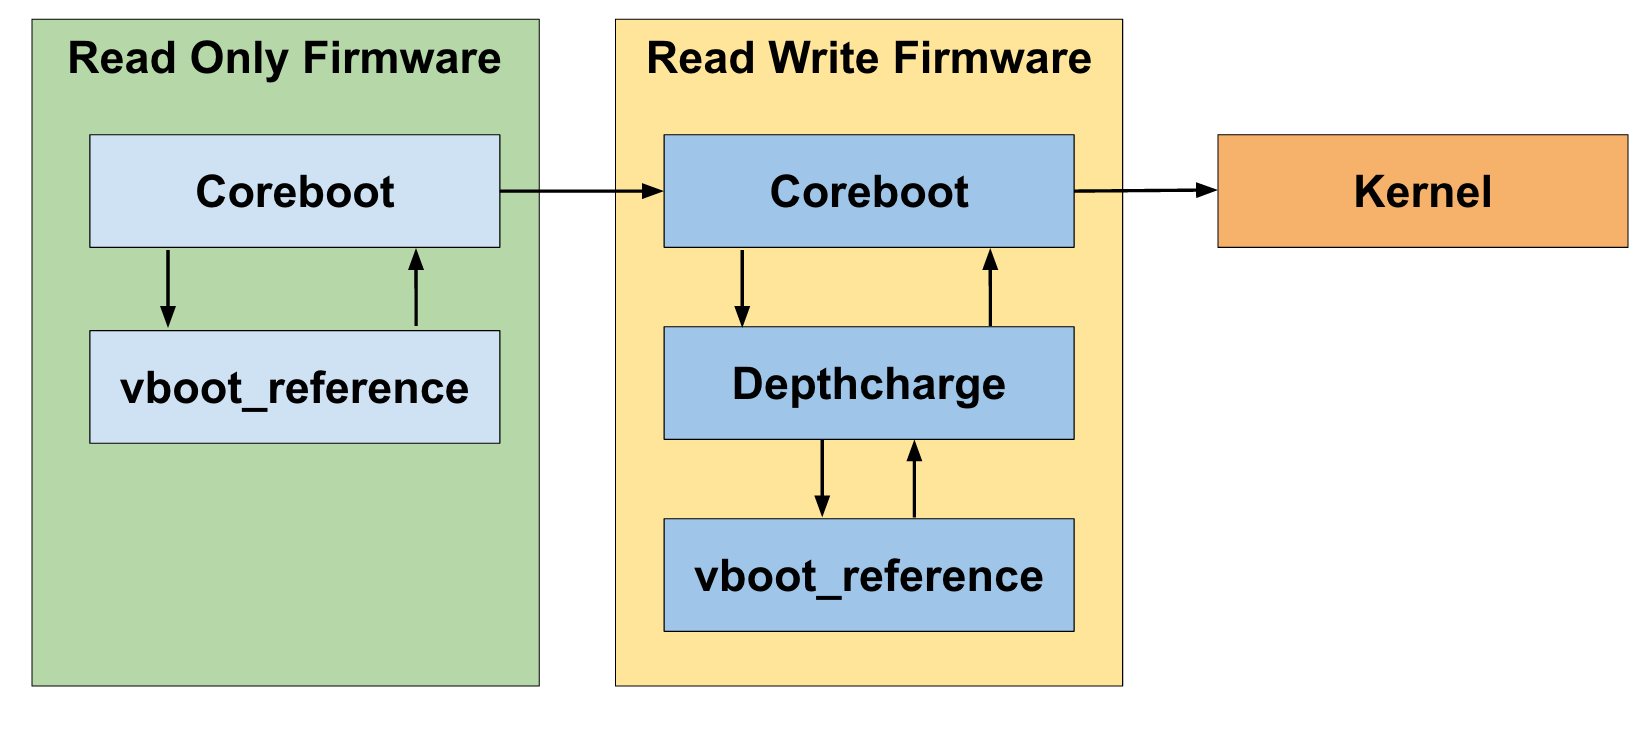
\includegraphics[width=0.8\linewidth]{code_repos}
  \caption{ChromeOS's boot flow goes through Coreboot, Depthcharge, and the Vboot Library twice for Firmware and Kernel verification}\label{fig:code_repos}
\end{figure}
\begin{figure}
  \centering
  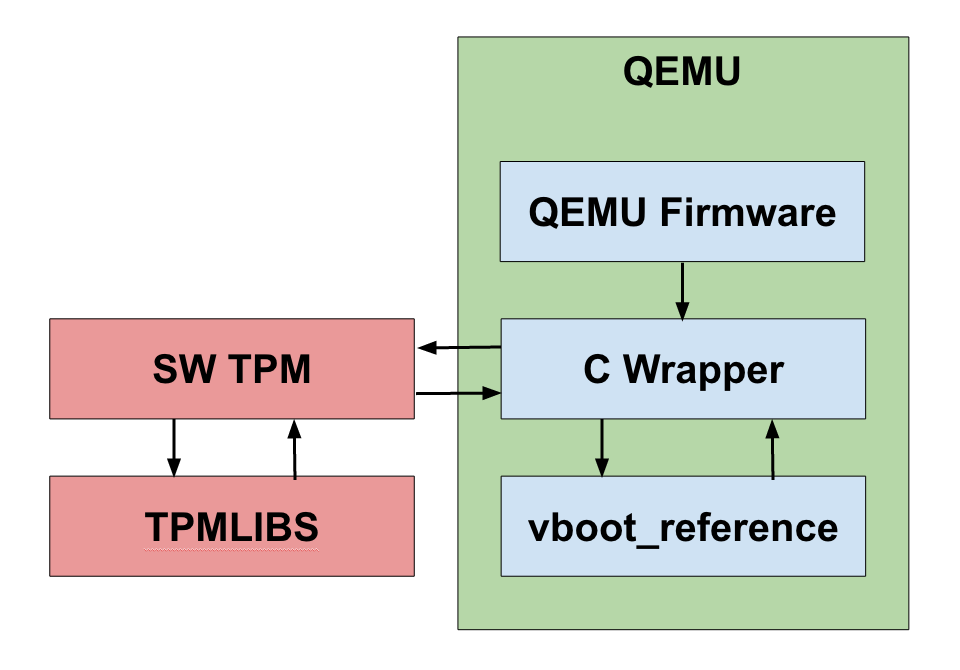
\includegraphics[width=0.45\linewidth]{qemu_repos}
  \caption{This report's boot flow uses QEMU's default bootloader Firmware, then
  a created C wrapper for the TPM and Debugging Output, and Vboot for the
  verification}\label{fig:qemu_repos}
\end{figure}

\subsection{Coreboot}\label{coreboot}

Coreboot is a fully Open-Sourced alternative to traditional BIOS implementations.~\cite{coreboot}
It is lightweight and is configured to implement the full standard of the Unified Extensible Firmware Interface (UEFI).
Google has chosen Coreboot because of its small code footprint, full extensibility, and the fact that it is available freely as an Open Source project.

The Coreboot code is responsible for doing very early initialization code on the main CPU\@. 
% This includes things like setting up the GPIO pins, enabling hardware interrupts, setting up a large stack in RAM, and providing driver callbacks to the payload that it will eventually call.
Coreboot is setup so that once a baseline level of initialization is complete, it passes control to another section of code called a ``payload''~\cite{coreboot-payload}.
This payload is responsible for initializing the more specialized drivers, and the concept of a payload means that Google can keep support more hardware without altering the Coreboot source code.
The payload that Coreboot calls to further initialize the Chromebook is Depthcharge.
% Init done in src/mainboard/google/{link}/romstage.c

\subsection{Vboot\_reference}

The vboot\_reference repo contains all of the control and algorithms for the vboot process~\cite{vboot-codebase}.
The repo is designed such that it does not rely on any knowledge about the platform.
If a function requires usage of a driver or something that is board specific, it will make a callback into Depthcharge which will provide the relevant information.

One of the more helpful features of the vboot\_reference repo is that it can be
built in a stand-alone fashion as a C archive file.
More information about building the project can be found in the appendix, but
this feature allowed the Vboot functions to be placed into the QEMU environment
easily, and it can be adapted for many different types of hardware.

\subsection{Software TPM}

This project uses a software-emulated TPM instead of a physical chip. 
This emulated TPM implements all of the TPM's functionality as defined by the
TCG Standards.
The fact that the emulation was software allowed the TPM to be put into various
states easily without requiring a physical reboot of the system.
Once the emulated TPM was passed to QEMU, it was accessed through the same
Memory Mapped Registers as the Hardware TPM outlined in Section~\ref{sec:TPM}.
This was very helpful because it meant that the Vboot TPM functions would work
with the emulated TPM.

The Software TPM was taken from a series of repositories created by IBM's
Stefan Berger. 
These repositories emulated the TPM functions\cite{TPMLibs}, the TPM Command
Fifo\cite{SWTPM}, and the TPM Register Interface\cite{TPMQEMU}. 
More information about installing the Software TPM libraries can be found in the
appendix.

\subsection{CBMC-Vboot}

The CBMC-Vboot is my personal repository for code\cite{my-repo}.
The layout of this repository is discussed in the Appendix.
We can see in Figure~\ref{fig:qemu_repos} that it is used as a wrapper to tie
Vboot together with QEMU and the SWTPM libraries.
It also holds python scripts which run the CBMC tests that I will describe in
Section~\ref{sec:Verif}.
